% 本章使用的 BibTeX 键：fusiello1998。

\section{相机矩阵的立体校正}
\label{sec:rectification-camera-matrices}

假设双目系统已经标定，即已知 PPM $\widetilde{P}_{o1}$ 和 $\widetilde{P}_{o2}$。立体校正的
基本思想是定义两个新的 PPM $\widetilde{P}_{n1}$ 和 $\widetilde{P}_{n2}$：将原相机绕其
光心旋转，直到两个焦平面共面并因此包含基线。这样可保证极点位于无穷远处，从而使对极线
彼此平行。为了使对极线水平，基线必须平行于两相机的新 $X$ 轴。此外，为了实现适当的
立体校正，共轭点必须具有相同的垂直坐标。这可以通过要求新相机具有相同的内参数来实现。
注意，由于焦距相同，成像平面也共面，如图~\ref{fig:rectified-cameras} 所示。

总而言之，新 PPM 的位置（即光心）与旧相机相同，而新的姿态（两台相机相同）通过适当的
旋转改变了旧姿态；两台相机的内参数也相同。因此，所得的两个 PPM 只在其光心上不同，
可以将它们看作一个沿其参考系 $X$ 轴平移的单个相机。

将新的 PPM 写成分解形式。由式~(2) 和式~(7) 得

\begin{equation}
  \widetilde{P}_{n1}=A[R\mid-Rc_1],\qquad
  \widetilde{P}_{n2}=A[R\mid-Rc_2]
  \label{eq:new-ppms}
\end{equation}

两个 PPM 使用相同的内参矩阵 $A$，且 $A$ 可以任意选取（见 MATLAB 代码）。光心 $c_1$
和 $c_2$ 就是由式~(6) 计算得到的旧相机光心。给出相机姿态的矩阵 $R$ 对两个 PPM
相同。下面用其行向量表示 $R$：

\begin{equation}
  R=\begin{bmatrix}r_1^{\mathsf T}\\r_2^{\mathsf T}\\r_3^{\mathsf T}\end{bmatrix}
  \label{eq:new-rotation-rows}
\end{equation}

它们分别是用世界坐标表示的相机参考系 $X$、$Y$、$Z$ 轴。

根据前述说明，取：

\begin{enumerate}
  \item 新 $X$ 轴平行于基线：
    \begin{equation*}
      r_1=\frac{c_1-c_2}{\lVert c_1-c_2\rVert}
    \end{equation*}
  \item 新 $Y$ 轴必须同时垂直于 $X$ 和 $k$：
    \begin{equation*}
      r_2=k\wedge r_1
    \end{equation*}
  \item 新 $Z$ 轴必须垂直于 $XY$：
    \begin{equation*}
      r_3=r_1\wedge r_2
    \end{equation*}
\end{enumerate}

在第 2 步中，$k$ 是任意单位向量，它确定新 $Y$ 轴在垂直于 $X$ 的平面中的位置。
取它为旧左相机矩阵的 $Z$ 轴单位向量，从而约束新 $Y$ 轴同时垂直于新 $X$ 轴和旧左
相机的 $Z$ 轴。

当光轴平行于基线时，即发生纯前向运动时，该算法会失效。

在 \citet{fusiello1998} 中，我们对立体校正要求进行了解析形式化，并证明了本节给出的
算法满足这些要求。

\begin{figure}[tb]
  \centering
  \IfFileExists{figures/fig2.png}{%
    \includegraphics[width=0.58\linewidth]{figures/fig2.png}%
  }{%
    \IfFileExists{task1/figures/fig2.png}{%
      \includegraphics[width=0.58\linewidth]{task1/figures/fig2.png}%
    }{%
      \fbox{\parbox[c][3.0cm][c]{0.72\linewidth}{\centering 图 2 原图待提取\\\small 路径：figures/fig2.png}}%
    }%
  }
  \caption{校正后的相机。成像平面共面且平行于基线。}
  \label{fig:rectified-cameras}
\end{figure}
